\documentclass[tikz,border=8pt]{standalone}
\usepackage{amsmath}
\usepackage{xcolor}
\definecolor{bgdark}{HTML}{171D2B}
\definecolor{gold}{HTML}{F7B538}
\definecolor{teal}{HTML}{4FD1C5}
\usetikzlibrary{calc}
\begin{document}
\pagecolor{bgdark}
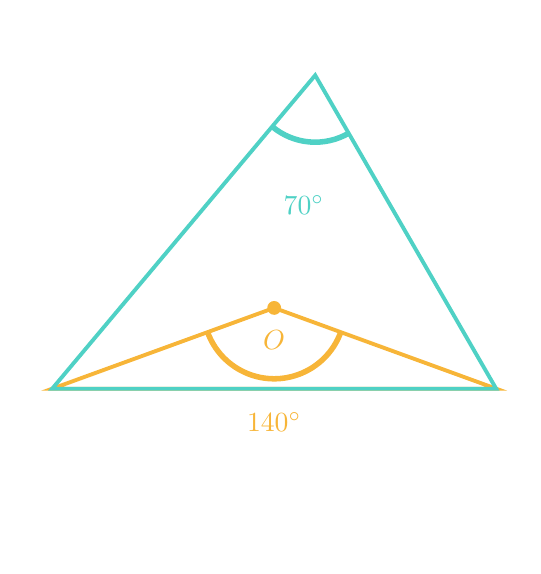
\begin{tikzpicture}[line width=1.4pt, text=white]
  % Lingkaran dan titik-titiknya
  \draw[white] (0,0) circle (3);
  \coordinate (O) at (0,0);
  \coordinate (A) at (200:3);
  \coordinate (B) at (340:3);
  \coordinate (C) at (80:3);
  \fill[gold] (O) circle (2.5pt) node[below=4pt] {$O$};
  \fill[white] (A) circle (2.5pt) node[anchor=95, inner sep=6pt] {$A$};
  \fill[white] (B) circle (2.5pt) node[anchor=35, inner sep=6pt] {$B$};
  \fill[white] (C) circle (2.5pt) node[above=3pt] {$C$};
  % Segitiga sudut pusat (emas)
  \draw[gold] (O) -- (A) -- (B) -- cycle;
  % Segitiga sudut keliling (hijau)
  \draw[teal] (C) -- (A) -- (B) -- cycle;
  % Busur sudut pusat 140 derajat
  \draw[gold, line width=2pt] (200:0.9) arc[start angle=200, end angle=340, radius=0.9];
  \node[gold] at (270:1.45) {$140^\circ$};
  % Busur sudut keliling 70 derajat di C
  \draw[teal, line width=2pt] ($(C)+(230:0.85)$) arc[start angle=230, end angle=300, radius=0.85];
  \node[teal] at ($(C)+(265:1.65)$) {$70^\circ$};
\end{tikzpicture}
\end{document}
